%%%%%%%%%%%%%%%%%%%%%%%%%%%%%%%%%%%%%%%%%
% Masters/Doctoral Thesis 
% LaTeX Template
% Version 1.43 (17/5/14)
%
% This template has been downloaded from:
% http://www.LaTeXTemplates.com
%
% Current author:
% Some items were added and modified by for use in 
% undergraduate Final Year Project (FYP) at
% Multimedia University, Cyberjaya, Malaysia.
% Wan Ruslan Yusoff 
% wruslan@mmu.edu.my
%
% Original authors:
% Steven Gunn 
% http://users.ecs.soton.ac.uk/srg/softwaretools/document/templates/
% and
% Sunil Patel
% http://www.sunilpatel.co.uk/thesis-template/
%
% License:
% CC BY-NC-SA 3.0 (http://creativecommons.org/licenses/by-nc-sa/3.0/)
%
% Note:
% Make sure to edit document variables in the Thesis.cls file
%
%%%%%%%%%%%%%%%%%%%%%%%%%%%%%%%%%%%%%%%%%
%----------------------------------------------------------------------------------------
%	PACKAGES AND OTHER DOCUMENT CONFIGURATIONS
%----------------------------------------------------------------------------------------

\documentclass[12pt, oneside]{Thesis} 
% The default font size and one-sided printing (no margin offsets)

\graphicspath{{Pictures/}} 
% Specifies the directory where pictures are stored
\usepackage{float} 
% To make picture stay at placement
\usepackage{pdfpages}
\usepackage{setspace} 
% Double spacing
%\doublespacing % Use on each page

\usepackage[square, numbers, comma, sort&compress]{natbib} 
% Use the natbib reference package - read up on this to edit the reference style; if you want text (e.g. Smith et al., 2012) for the in-text references (instead of numbers), remove 'numbers' 

\hypersetup{urlcolor=black, colorlinks=true} 
% Colors hyperlinks in blue - change to black if annoying

\title{\ttitle} 
% Defines the thesis title - don't touch this

% ================================================
% % ADDED BY WRY
\usepackage{caption}
\usepackage{appendix}
\usepackage{tikz}
\usepackage[europeanresistors,americaninductors]{circuitikz}
\usetikzlibrary{chains}
% ==================================================
\begin{document}
% ==================================================


\frontmatter 
% Use roman page numbering style (i, ii, iii, iv...) for the pre-content pages

\setstretch{1.3} 
% Line spacing of 1.3

% Define the page headers using the FancyHdr package and set up for one-sided printing
\fancyhead{} 
% Clears all page headers and footers
\rhead{\thepage} 
% Sets the right side header to show the page number
\lhead{} 
% Clears the left side page header

\pagestyle{fancy} 
% Finally, use the "fancy" page style to implement the FancyHdr headers

\newcommand{\HRule}{\rule{\linewidth}{0.5mm}} 
% New command to make the lines in the title page

% PDF meta-data
\hypersetup{pdftitle={\ttitle}}
\hypersetup{pdfsubject=\subjectname}
\hypersetup{pdfauthor=\authornames}
\hypersetup{pdfkeywords=\keywordnames}

%----------------------------------------------------------------------------------------
%	TITLE PAGE
%----------------------------------------------------------------------------------------

\begin{titlepage}
\begin{center}

{\LARGE \ttitle}\\[0.4cm] 
\vfill
\Large{Zeiyad Fathi Sfaxsi, Mahmood Sarzil, Karishma Patel A/P Balvantry} 

\vfill
\normalsize{SESSION 2016}
\vfill
\normalsize\FACNAME\\
\normalsize \UNIVNAME\\
{\normalsize MAY 2016}\\ 
\vfill
\end{center}

\end{titlepage}
\thispagestyle{empty}
\begin{center}

	{\LARGE \ttitle}\\[0.4cm] % Thesis title
	\vfill
	\footnotesize{BY}
	\vfill
	\Large{Zeiyad Fathi Sfaxsi, Mahmood Sarzil, Karishma Patel A/P Balvantry} % Author name - remove the \href bracket to remove the link
	\vfill
	\footnotesize{SESSION 2016}
	\vfill
	\footnotesize{THIS PROJECT REPORT IS PREPARED FOR}
	\vfil
	\normalsize\FACNAME\\
	\normalsize \UNIVNAME\\
	\normalsize{IN PARTIAL FULFILLMENT}\\
	\normalsize{FOR}\\
	\vfil
	\normalsize{BACHELOR OF COMPUTER SCIENCE (HONS)}\\
	\normalsize{WITH SPECIALIZATION IN}\\
	\normalsize{INFORMATION SYSTEMS}\\
	\vfil
	\normalsize\FACNAME\\
	\vfil
	\Large \UNIVNAME\\
	\vfil
	{\normalsize MAY 2016}\\ % Date
	%\includegraphics{Logo} % University/department logo - uncomment to place it
	\vfill
\end{center}

\newpage
\thispagestyle{empty}

The copyright of this thesis belongs to the author under the terms of the Copyright Act 1987 as qualified by Regulation 4(1) of the Multimedia University Intellectual Property Regulations. Due acknowledgment shall always be made of the use of any material contained in, or derived from, this thesis. 

\vfil
\textit{© The Killers, 2016}\\
All rights reserved


%----------------------------------------------------------------------------------------
%	DECLARATION PAGE
%	Your institution may give you a different text to place here
%----------------------------------------------------------------------------------------
\newpage
\Declaration{

\addtocontents{toc}{\vspace{1em}} 
% Add a gap in the Contents, for aesthetics

I hereby declare that the work in this thesis have been done by myself and no portion of the work contained in this thesis has been submitted in support of any application for any other degree or qualification of this or any other university or institute of learning.

\vfill

\rule[1em]{25em}{0.5pt} % This prints a line for the signature
\\\textit{The Killers}
\\Faculty of Computing \& Informatics
\\Multimedia University
\\Date: 17$^{th}$ May 2016

}

\clearpage % Start a new page

%----------------------------------------------------------------------------------------
%	ACKNOWLEDGEMENTS
%----------------------------------------------------------------------------------------

\setstretch{1.3} % Reset the line-spacing to 1.3 for body text (if it has changed)

\acknowledgements{\addtocontents{toc}{\vspace{1em}} % Add a gap in the Contents, for aesthetics
\begin{flushleft}
\doublespacing

We would like to express our deepest appreciation to all those who provided us the possibility to complete this report.  A special gratitude we give to our lecturer, Mr. Wan Ruslan Yusoff, whose contribution in stimulating suggestions and encouragement,  helped us to coordinate our project especially in learning and practicing software engineering principles and activities.\\ 


Furthermore we would also like to acknowledge with much appreciation the senior students, who helped us by providing us with their experience.\\

 A special thanks goes to our friends, who  helped us by assembling the parts and giving suggestions about the task.\\
 
Many thanks go to our parents who are the reason of us being able to study in  MMU. Moreover, they have invested their full effort in guiding us in achieving our goals.\\
 
  Last but not least, we have to appreciate the guidance given by other lecturers as well as the workers especially in the faculty of computing and informatics.

\end{flushleft}
}
\clearpage % Start a new page

%----------------------------------------------------------------------------------------
%	LIST OF CONTENTS/FIGURES/TABLES PAGES
%----------------------------------------------------------------------------------------

\pagestyle{fancy} % The page style headers have been "empty" all this time, now use the "fancy" headers as defined before to bring them back

\lhead{\emph{Contents}} % Set the left side page header to "Contents"
\tableofcontents % Write out the Table of Contents

\lhead{\emph{List of Figures}} % Set the left side page header to "List of Figures"
\listoffigures % Write out the List of Figures

\lhead{\emph{List of Tables}} % Set the left side page header to "List of Tables"
\listoftables % Write out the List of Tables

% ADDED BY WRY
%% AUTOMATIC LIST OF LISTINGS
% \phantomsection
% \addtotoc{List of Software Codes}
\lhead{\emph{List of Software Codes}}
\lstlistoflistings


%----------------------------------------------------------------------------------------
%	ABBREVIATIONS AND ACRONYMS 
%----------------------------------------------------------------------------------------
% ADDED BY WRY
\pagebreak
\addtotoc{Abbreviations and Acronyms} 
\lhead{\normalfont\huge{Abbreviations and Acronyms}}


% TABLE HEADER
\begin{table}[ht]
\begin{tabular}{p{2.5cm}p{11.0cm}}
% ========================================

\textbf{FCI} & Faculty of Computing and Informatics\\
\textbf{MMU} & Multimedia University\\
\textbf{MTS} & My Transportation Schedule (Software name)\\
\textbf{Q.A.} & Quality Assurance\\
% ======================================
\end{tabular}
\end{table}


% ======================================
%	ABSTRACT PAGE 
% ADDED BY WRY
\pagebreak
\addtotoc{Management Summary} 
\lhead{\normalfont\huge{Management Summary}}

%\vspace*{1\baselineskip}
Procedural design is considered the low level algorithmic design of software codes or computer programs. It covers the design of procedures, that is, the inner details of the steps and instructions the program are to execute to achieve their intended objectives. 

% \vspace*{1\baselineskip}
Procedural design activities can also be interpreted as the design activities at the level of software components. The software constructor will use these procedural designs and write software codes to implement and execute those designs. 



\clearpage % Start a new page
\pagebreak
%----------------------------------------------------------------------------------------
%	THESIS CONTENT - CHAPTERS
%----------------------------------------------------------------------------------------

\mainmatter 
% Begin numeric (1,2,3...) page numbering

\pagestyle{fancy} 
% Return the page headers back to the "fancy" style

\raggedright
\chapter{Software Project Planning} 
% Main chapter title

\label{Chapter1} 
%Call reference to this chapter use \ref{ChapterX}

\lhead{Chapter 1. \emph{Software Project Planning}} 
% Change X to a consecutive number; this is for the header on each page - perhaps a shortened title

\doublespacing
% LINE FORMATTING

%\clearpage
%\pagebreak

% MAIN SECTION ==============================
\section{Introduction}

\subsection{Project Brief Description}
MTS (My Transportation Schedule) is a daily activity application that could be installed in any Android (An operating system works in mobiles and tablets) device. It focuses on the people who are using the public transportation system in Cyberjaya.\\

The buses among cyberjaya will be provided by a GPS tracker that would track the bus and update the database. The user will be able to organize his timetable through MTS.\\ 

The user is only required to insert the time, the date and location in Cyberjaya of the event, MTS garanties that the user will not be late on any event, by choosing the best route considering the density as well as the traffic. MTS is designed to be able to alarm the user if the target destination cannot be reached on time.

\subsection{MTS is an IoT Software}
Internet of Things (IoT) is a connection of physical objects such as devices, buildings, vehicles, and items embedded through electronics, sensors, softwares, and network connectivity that are allowing all these items to get and exchange data \cite{wikiIOT}.\\

A GPS device is considered as a sensor for tracking the object’s location which is one of the main necessity for an IoT application \cite{second}.\\

Our software uses GPS trackers that are installed to the buses that allows the exchange of data. The software, connects through the GPS with the use of a sim card that allows the GPS to connect to the server that transfers data \cite{third}.\\

\subsection{Project Objectives}
\begin{itemize}
	\item Minimizing the chance of being late. 
	\item Avoid wasting time waiting in the bus station for the bus to come.
	\item Build a software with a good user experience (UX).
\end{itemize}


\pagebreak
%MAIN SECTION ================================
\section{Project Scope}
MTS covers only buses in Cyberjaya. For further prototypes, MTS might be extended to have a wider coverage and more public transportation methods such as trains and Taxis.\\

For starting prototypes, MTS has only four engineers working on it. Which leads to make the starting prototypes used by only few hundreds users to ease the proccess of finding and fixing bugs.\\

For the first prototypes, the application would be bassed on Android operation system. \\

\section{Installation}
MTS needs two servers that are the main server and the backup server to be installed. The backup server will be a copy of the main server. The backup server will be in service automatically if the main server stopped working. Figure \ref{fig:ServerArch} shows the relationship between servers and their databases.

\begin{figure}[H]
	\centering
	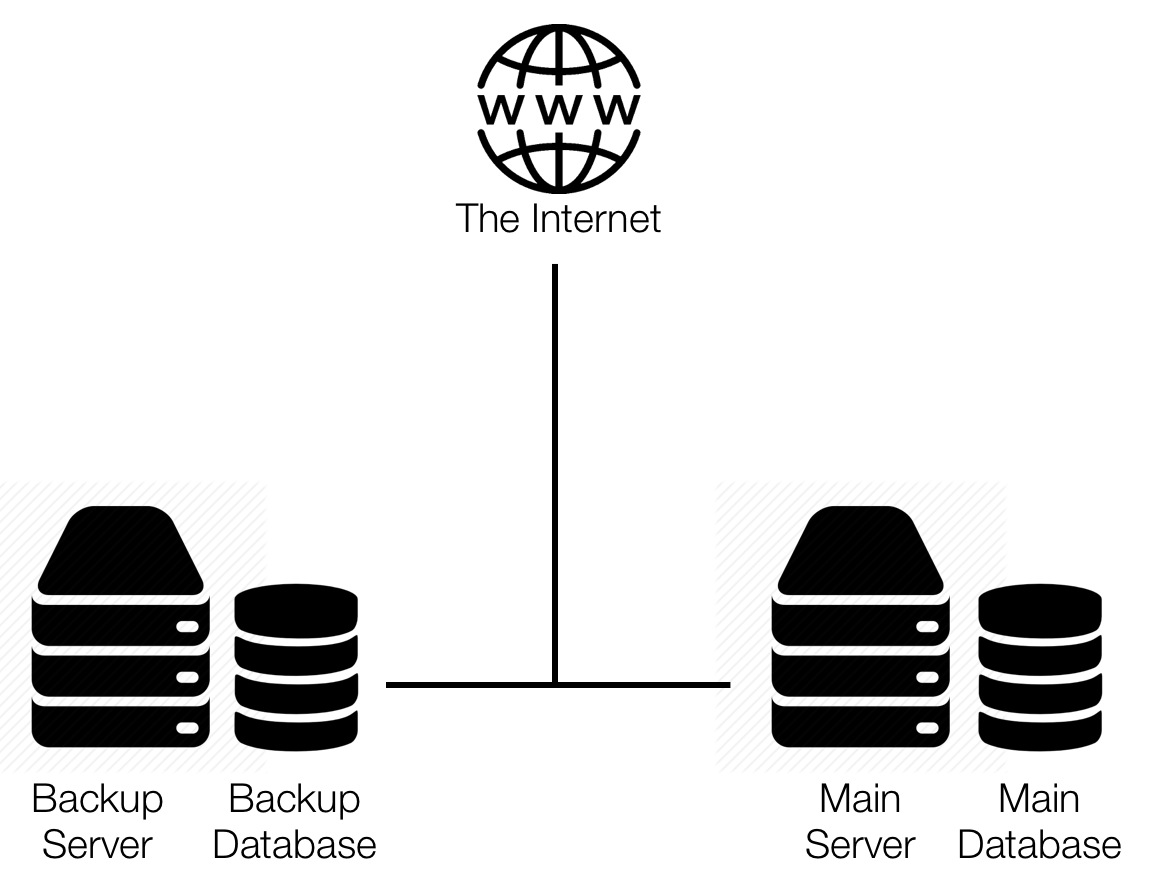
\includegraphics[scale=0.55]{Figures/FigureInstallation.png}
	\rule{35em}{0.5pt}
	\caption[Gantt Chart: Estimated Timeline for a prototype]{Gantt Chart: Estimated Timeline for a prototype}
	\label{fig:ServerArch}
\end{figure}

A chip equipped with a GPS tracker and a SIM card will be installed to every public transportation bus in cyberjaya. The GPS tracker will manage the location tracking function which gets every bus’s location from the GPS  Satellite and update it in the database, while the sim card will be providing the chip with the Internet connection.\\

\section{Execution}
The first two prototypes will be available only for the developers; For the sake of developing and improving. MTS will be available in Google Play after the release of the third prototype. For the ease of testing the prototype, 200 users will be capable of using MTS by then. However, the software will be available for all cyberjaya users after the delivery of the fifth prototype.\\

During execution, feedbacks will be noted from stakeholders in order to list the following prototype’s requirements.


\section{Feedbacks and updates}
At the first two prototypes the developers will list their feedbacks. By the third prototype the users will be able to use and give their feedback about MTS. A feedback is considered as soon as it’s received and the update will be held to the next prototype to be out.



\pagebreak
 % INTRODUCTION - PROJECT OBJECTIVES/PROBLEM STATEMENTS
\chapter{Estimated Budget} 
% Main chapter title

\label{Chapter2} 
%Call reference to this chapter use \ref{ChapterX}

\lhead{Chapter 1. \emph{Estimated Budget}} 
% Change X to a consecutive number; this is for the header on each page - perhaps a shortened title

\doublespacing
% LINE FORMATTING

% MAIN SECTION ==============================
\section{Hardware itmes cost}
Below is a table of items needed and it's prices.

\begin{table}[ht]
	\begin{center}
		\begin{tabular}{ |p{1.5cm}|p{3cm}|p{3cm}|p{4cm}|p{1.5cm}| }
			\hline \multicolumn{5}{|c|}{\textbf{Items needed for the project}} \\ [1.0ex]
			\hline \textbf{Item} & \textbf{Description} & \textbf{Alternative} & 
			\textbf{Purpose of choose} & \textbf{Price} \\
			\hline CPU & Intel Xeon  & AMD Athlon
			 & Cost & 389.39\$  \\ 
			\hline RAM & Kingston 
			16 GB  &  Corsair
			16 GB  & Quality  & 76.39\$\\ 
			\hline HDD & Seagat 1 TB
			  & Kingsnot 1 TB & Cost  & 49.99\$  \\ 
			\hline GPS tracker & Hossenchip  & HCT Micro
			 & Cost  & 16.99\$  \\ 
			 \hline SSL certificate & PositiveSSL from SSLs.com & godaddy
			 & Cost  & 4.99\$  \\ 
			 
			\hline Others & Keyboard, Mouse, screen … etc     & - & - & 290\$ \\
			\hline  Total & & & &727.75\$ \\
			\hline
			
		\end{tabular}
		
		\caption{Items needed for the project}
		\label{table:Itmes-needed-for-project}
	\end{center}
\end{table}

Because we are going to use two servers - main and backup servers - the cost would be \textbf{1421.52\$}\\

Cyberjaya has aproxmatily thirty-six buses price of GPS tracker multiplayed with thirty-six has to be added. The total price of GPS tracker is \textbf{611.64\$}.


Total cost is \textbf{2033.16\$}. % LITERATURE SURVEY
\chapter{Estimated Timeline} 
% Main chapter title

\label{Chapter3} 
%Call reference to this chapter use \ref{ChapterX}

\lhead{Chapter 3. \emph{Estimated Timeline}} 
% Change X to a consecutive number; this is for the header on each page - perhaps a shortened title

\doublespacing
% LINE FORMATTING

\section{Estimated Timeline}
Because MTS will be developed by using prototyping model, It is estimated that the thired prototype would be stable enough to be published in the Google Play - The market of android's applications -.\linebreak \\

The second and first prototype are to find bugs and security issues in earlier time which reduce the risk and minimize the cost of fixing.\linebreak \\

Each prototype needs at least twenty-one weeks to be fully deployed. Furthermore, the work of a following prototype would be established on the nineteenth week of previous prototype. \\

\pagebreak

\subsection{Gantt Chart}

Below the Gantt Chart discripes estimated timeline for each prototype.\\

\begin{figure}[H]
	\centering
	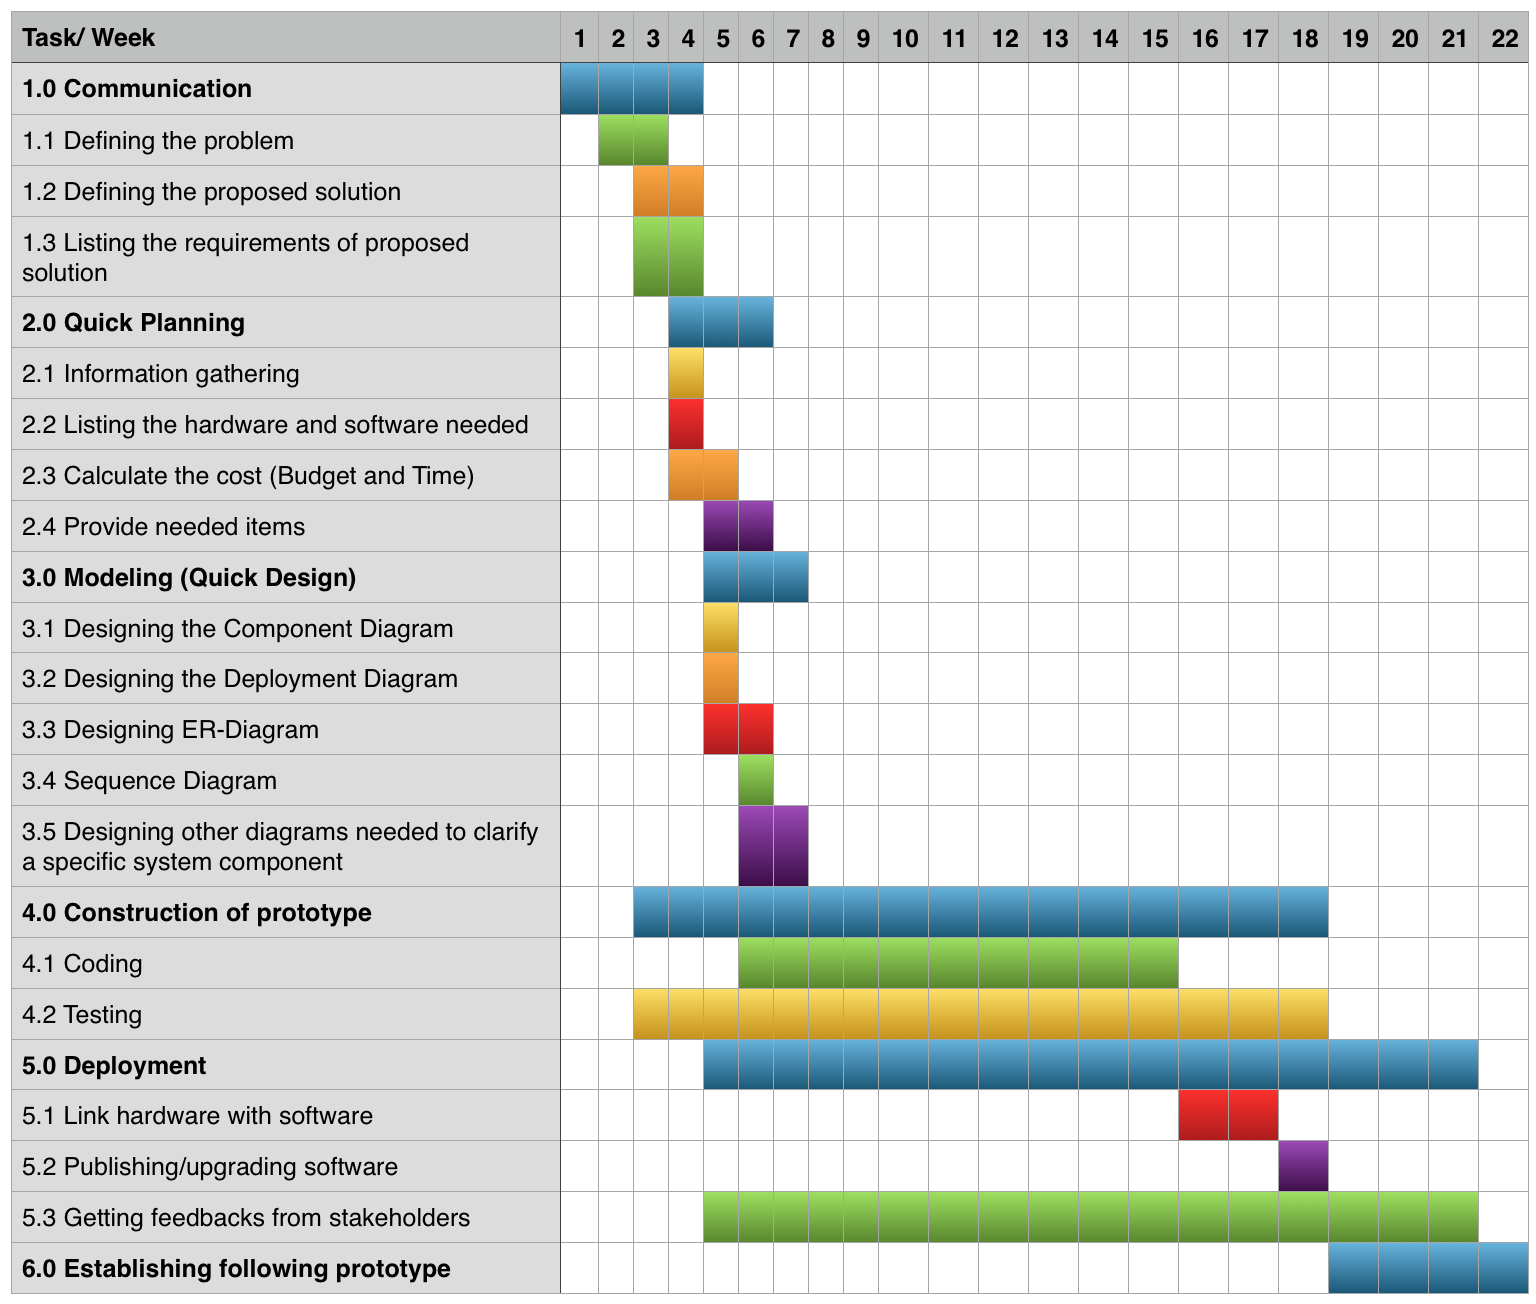
\includegraphics[scale=0.55]{Figures/FigureGanttChart.png}
	\rule{35em}{0.5pt}
	\caption[Gantt Chart: Estimated Timeline for a prototype]{Gantt Chart: Estimated Timeline for a prototype}
\end{figure}




%\clearpage
%\pagebreak

 % IMPLEMENTATION METHODOLOGY/PROPOSAL DESIGN
\chapter{Project Organization and Structure} 
% Main chapter title

\label{Chapter4} 
%Call reference to this chapter use \ref{ChapterX}

\lhead{Chapter 4. \emph{Project Organization and Structure}} 
% Change X to a consecutive number; this is for the header on each page - perhaps a shortened title

\doublespacing
% LINE FORMATTING

%\clearpage
%\pagebreak

% MAIN SECTION ==============================
\section{Manpower}
This project is handled by four Software engineering students. That leads everyone to handle more than one position which produce a higher quality product after each prototype.
\pagebreak
\section{Project Organization and Structure}
Team members are having a role rotation plan that designed to enhance the product by team members abilities. Below is the organization chart shows basic roles:
\begin{figure}[H]
	\centering
	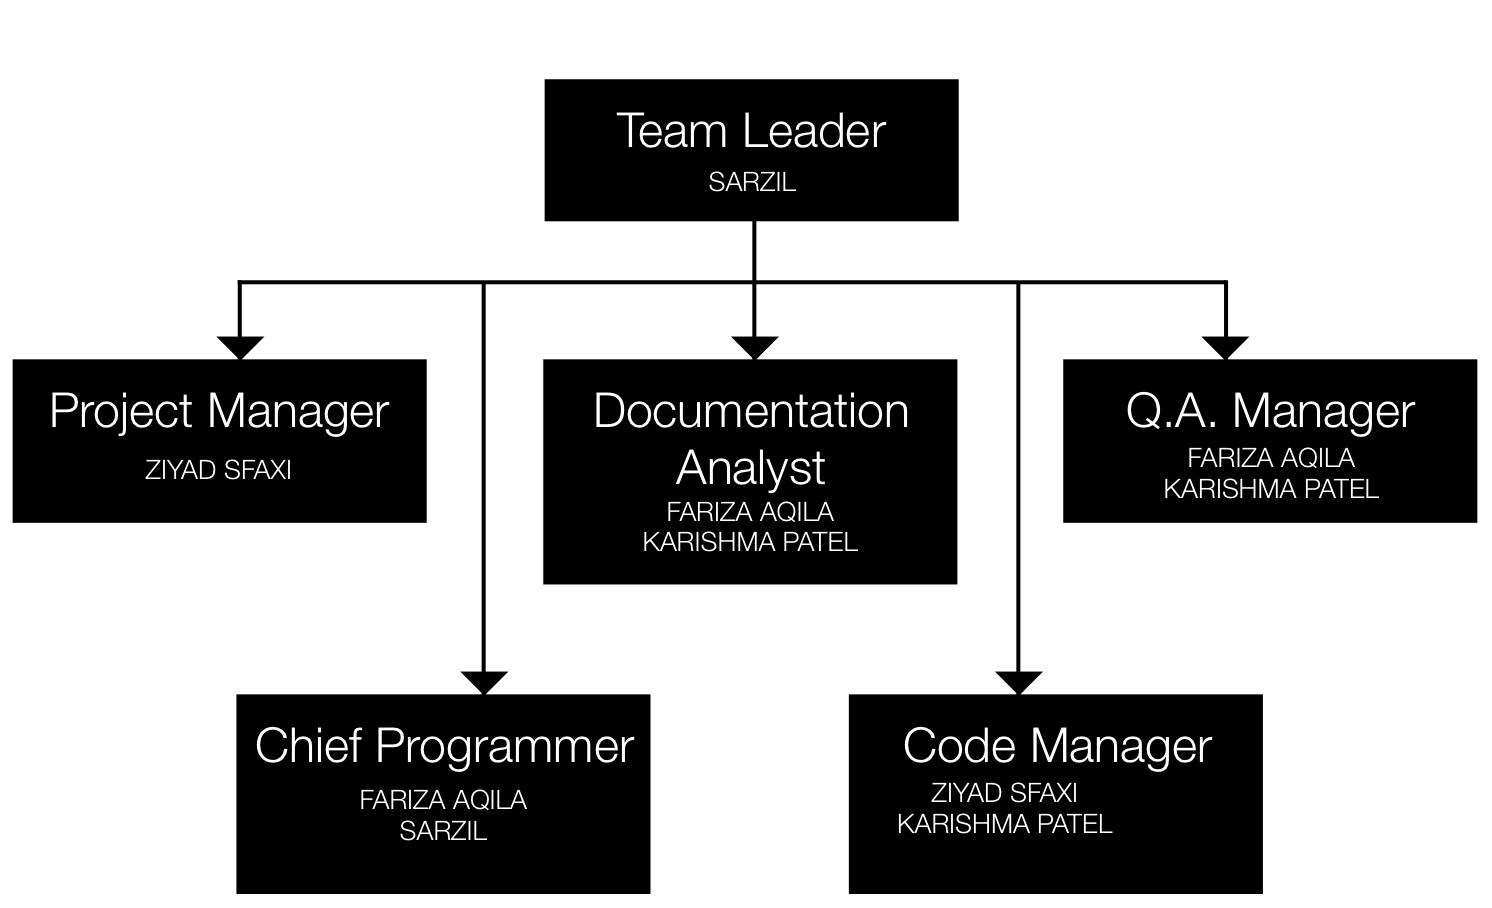
\includegraphics[scale=0.5]{Figures/FigureOrganizationChart.png}
	\rule{35em}{0.5pt}
	\caption[Organization Chart]{Organization Chart}
\end{figure}
\pagebreak

Below is a table that descripe every role:

\begin{table}[H]
	\centering
	\begin{tabular}{|p{4cm}|p{9.5cm}|}
		\hline
		{\bf ORGANIZATION}             & \bf DESCRIPTION                              \\ \hline
		{\bf Team Leader}           &  \begin{itemize}
			\item Serve as main contact with the managers.
			\item Ensuring the team is consistently delivering working software to the standards the department expects.
			\item Ensuring the team is self-organising so that we take collective responsibility for the work we do.
		\end{itemize}\\ \hline
		{\bf Project Manager} & \begin{itemize}
			\item Rotate roles to maximize the result of team abilities.
			\item Coordinate all those resources and the team’s tasks – to make sure that work is done in the proper sequence with a minimum of time.
			\item Ensuring the scope project is delivered and the body of  work is accomplished.
		\end{itemize}\\ \hline
		 \end{tabular}\end{table}
	\pagebreak \clearpage
	\begin{table}[H]
	\begin{tabular}{|p{4cm}|p{9.5cm}|}
		\hline
		{\bf Q.A. Manager}           &  \begin{itemize}
			\item Assures the viability, functionality and effectioness of essential tools.
			\item Anticipates program release problems and takes coorective action, escalation as needed, to resolve and achieve commitments.
		\end{itemize}\\ \hline
		{\bf Documentation
			Analyst}& \begin{itemize}
			\item Ensure that all documents have no errors in filenames or submissions.
			\item Perform evaluations and document audits.
		\end{itemize}\\ \hline
		
		{\bf Chief Programmer}  &  Convert the design and to a programming langauge.\\ \hline
		{\bf Code Manager} & Maintain the record of code files and the make file(s)\\ \hline

	\end{tabular}
	\caption{Table of organization roles}
	\label{Table of organization roles}
\end{table}
 % IMPLEMENTATION PLAN
\chapter{Software Process Model} 
% Main chapter title

\label{Chapter5} 
%Call reference to this chapter use \ref{ChapterX}

\lhead{Chapter 5. \emph{Software Process Model}} 
% Change X to a consecutive number; this is for the header on each page - perhaps a shortened title

\doublespacing
% LINE FORMATTING

%\clearpage
%\pagebreak

% MAIN SECTION ==============================
\section{Prototyping model}
\subsection{Description}
Prototyping model has five main phases which are listed below:
\begin{description}
	\item[Communication:] Gathering and discusing the requirements from and with users.
	\item[Quick Planning:] Establishes a plan for software engneering work, addresses technical tasks, resources, work products, and work schedule.
	\item[Modeling (Quick Desgin):] A quick plan that brings together customer requirements, business needs and technical considerations.
	\item[Construction of prototype:] Combines code generation and testing uncover errors.
	\item[Deployment, Delivery, and Feedback:] Involves delivery of software to the customers (Users) evalution and feedback.
\end{description}

\begin{figure}[H]
	\centering
	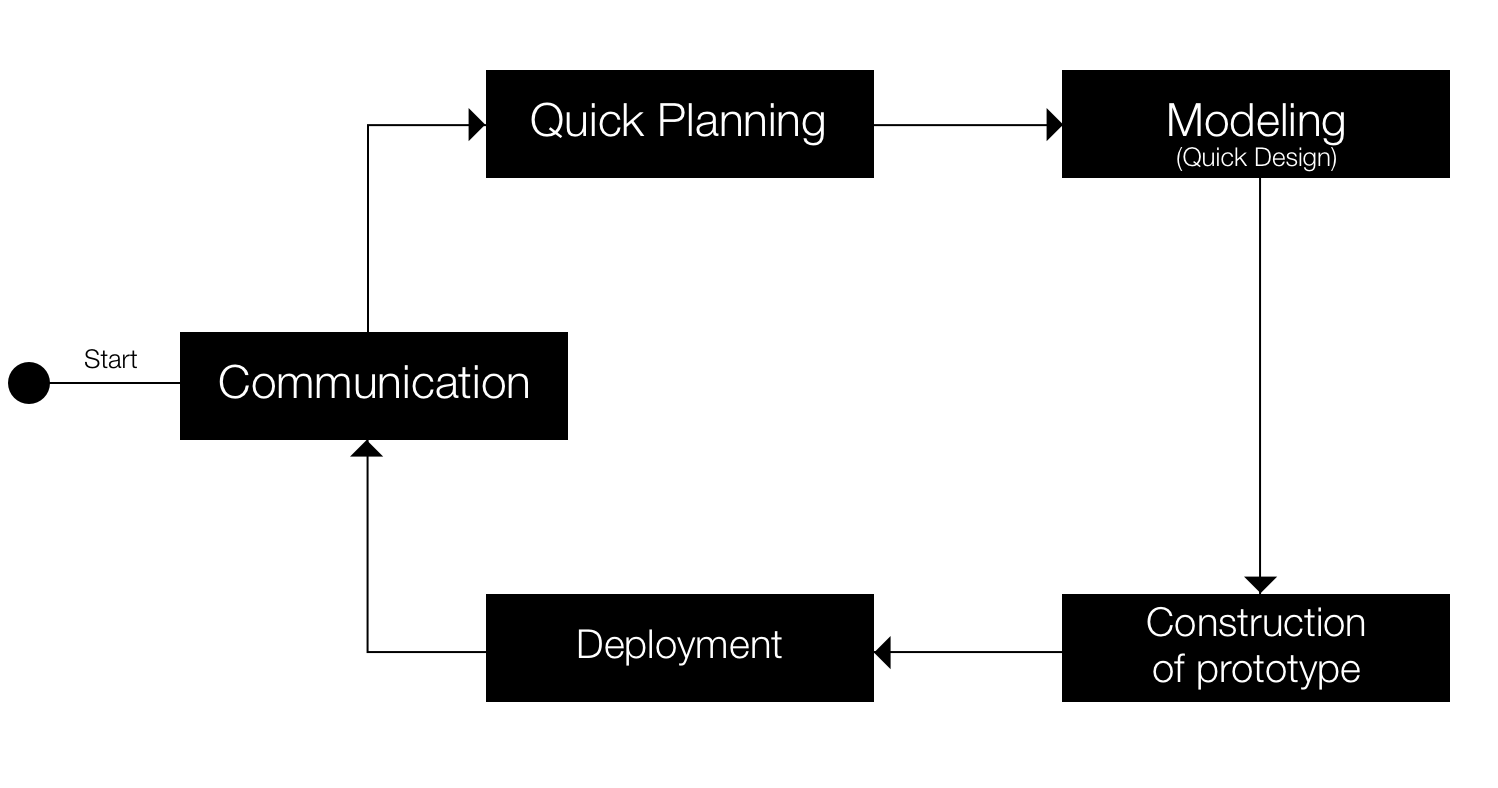
\includegraphics[scale=0.5]{Figures/PrototypingModel.png}
	\rule{35em}{0.5pt}
	\caption[Prototype Model Diagram]{Prototype Model Diagram}
\end{figure}

\pagebreak
\subsection{Reasons for choosing prototyping model}
By end of 2016 the population in Cyberjaya will be about 100,00, and most of people in Cyberjaya uses buses as their cheap and easy transportation method \cite{ReferencePopulationOfCyberjaya}. That makes MTS highly required and might be used by most of people who live in Cyberjaya. For that reason, bugs would be found easily and bugs would need a quick fix to reduce the damages and failures.\\

An advantage of Prototyping model is that the quicker user feedback is available which leads to better solutions and fast error fixing. In other words, users are actively involved in the development.\\

MTS is an system that needs to have interactions with the end users, therefore, Prototype model should be used. Moreover, MTS is an online system which has direct interfaces with many users at the same time. MTS might has a high amount of interaction with the end-users so prototype model is best compared to other models.\\ % RESULTS AND FINDINGS
\chapter{Software Components or Modules needed} 
% Main chapter title

\label{Chapter6} 
%Call reference to this chapter use \ref{ChapterX}

\lhead{Chapter 6. \emph{Software Components or Modules needed}} 
% Change X to a consecutive number; this is for the header on each page - perhaps a shortened title

\doublespacing
% LINE FORMATTING

%\clearpage
%\pagebreak
\section{Software Components and Modules needed}
Below the list that shows and, descripe components and modules needed to build MTS.

\begin{description}
	\item[Web server] description
	\item[Backup server] description
	\item[Database] description
	
\end{description}

% MAIN SECTION ==============================
\pagebreak
\section{Software Architecture}
Below is an architecture diagram shows the software architecture.
\begin{figure}[H]
	\centering
	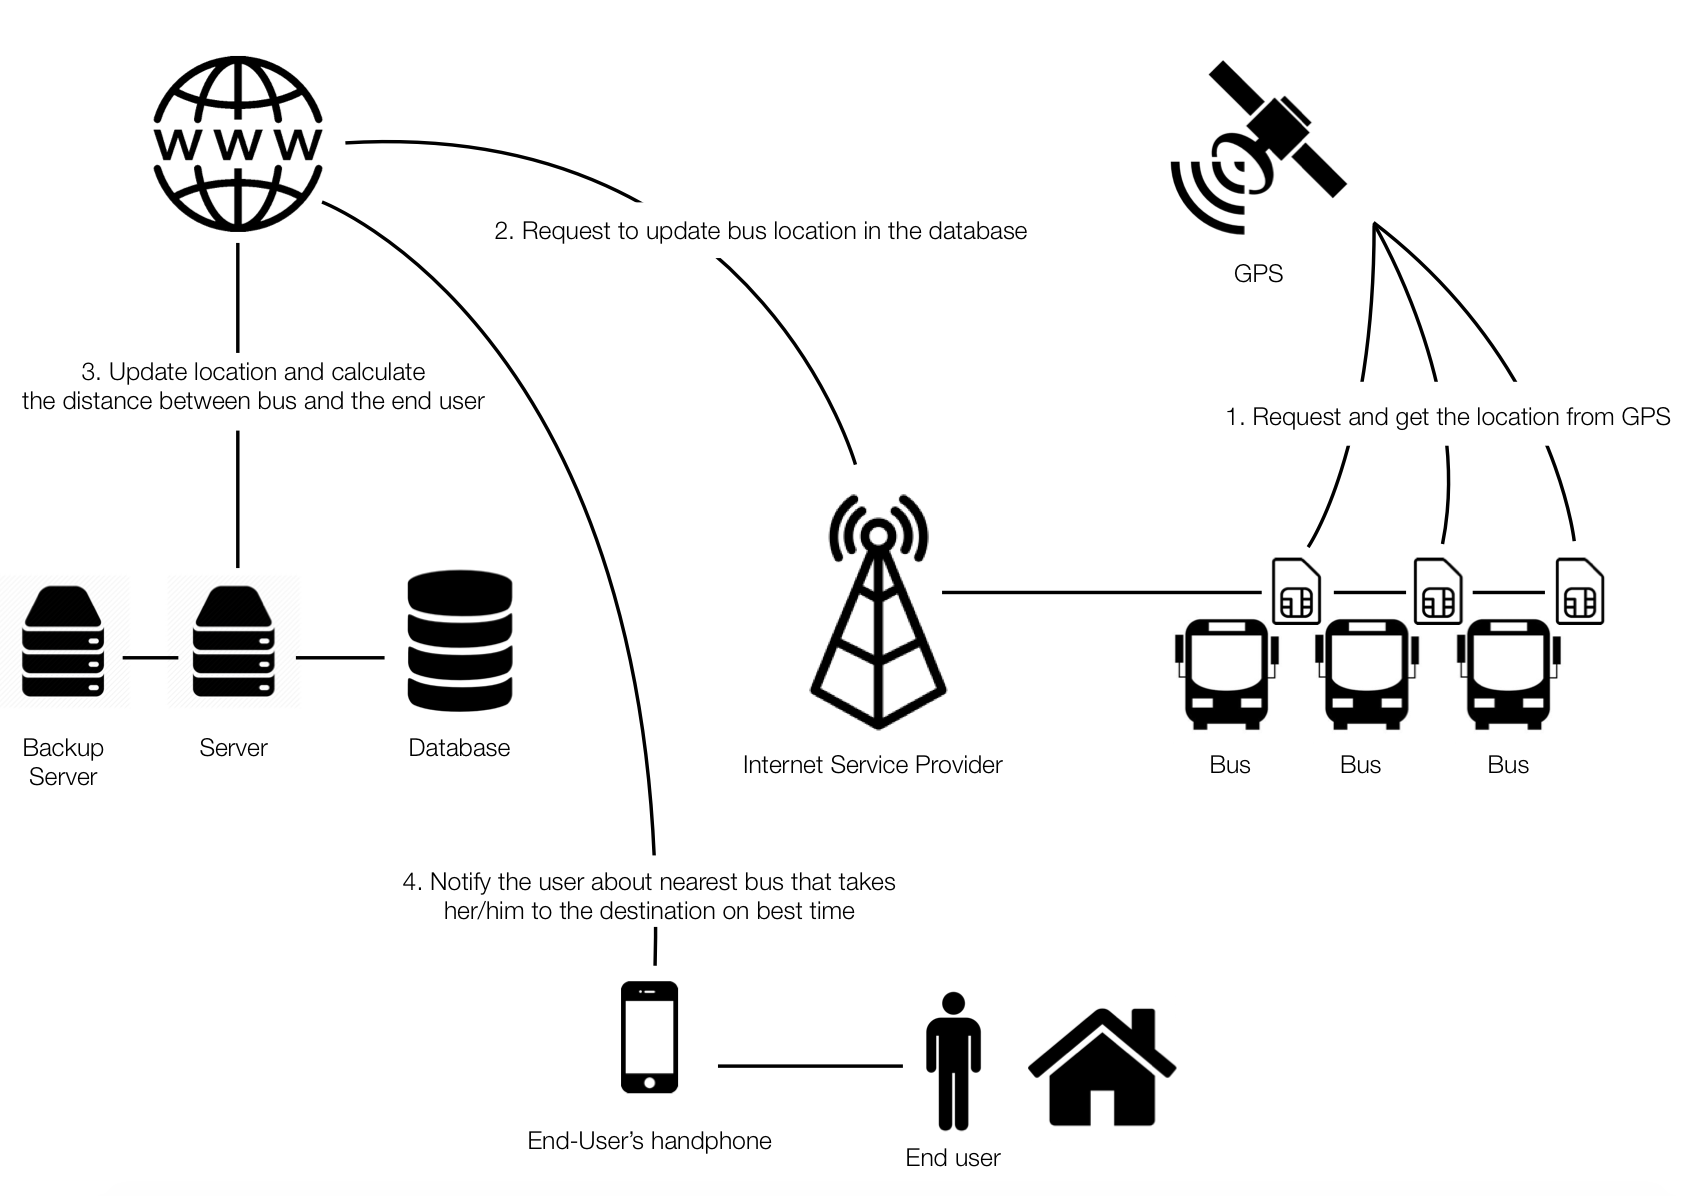
\includegraphics[scale=0.5]{Figures/FigureProposedSoftwareArchitecture.png}
	\rule{35em}{0.5pt}
	\caption[Software Architecture]{Software Architecture}
\end{figure}
\pagebreak
 % DISCUSSIONS AND RECOMMENDATIONS
\chapter{Conclusions} 
% Main chapter title

\label{Chapter7} 
%Call reference to this chapter use \ref{ChapterX}

\lhead{Chapter 7. \emph{Conclusions}} 
% Change X to a consecutive number; this is for the header on each page - perhaps a shortened title

\doublespacing
% LINE FORMATTING

%\clearpage
%\pagebreak

% MAIN SECTION ==============================
\section{Conclusions}

\section{Recommendations for Future Work}

Conclusions
Recommendations for Future Work

 % CONCLUSIONS


\clearpage

% ====================================
%	BIBLIOGRAPHY
\label{Bibliography}

\lhead{\emph{Bibliography}} 
% Change the page header to say "Bibliography"

\bibliographystyle{unsrtnat} 
% Use the "unsrtnat" BibTeX style for formatting the Bibliography

\bibliography{Bibliography} 
% The references (bibliography) information are stored in the file named "Bibliography.bib"

% ====================================
\addtocontents{toc}{\vspace{2em}} 
% Add a gap in the Contents, for aesthetics

\appendix
%\appendixpage
%\addappheadtotoc

\singlespacing  % USE SINGLE SPACING FOR APPENDICES

\chapter{Settings in the Preamble Section} 
% Main appendix title

\label{AppendixA} 
% Change X to a consecutive letter; for referencing this appendix elsewhere, use \ref{AppendixX}

\lhead{Appendix A. \emph{Settings in the Preamble Section}} 
% Change X to a consecutive letter; this is for the header on each page - perhaps a shortened title

% Write your Appendix content below here.
% =========================================

\section{Section Title}
To understand the basic ideas of software design Add and remove tabs Working with tabs in gedit allows you to keep an eye on several \index{files} in a single window. 

\subsection{subsection title}
The tab that is larger than the other tabs \index{indicates} the file that is currently open. The smaller tabs indicate other files that are available to work on. 

\subsection{subsection title}
To understand the place of software in software engineering What is design? What is Software Design? 


\chapter{Inserting Inline Tables} 
\label{AppendixB} 
\lhead{Appendix B. \emph{Inserting Inline Tables}} 

% Write your Appendix content below here.
% =========================================

\section{Section Title}
To understand the basic ideas of software design Add and remove tabs Working with tabs in gedit allows you to keep an eye on several \index{files} in a single window. 

\begin{table}[ht]
\begin{center}
\begin{tabular}{ |p{1.5cm}|p{2cm}|p{2cm}|p{5cm}|p{1.5cm}| }
\hline \multicolumn{5}{|c|}{\textbf{TUTORIAL SECTIONS SCHEDULE}} \\ [1.0ex]
\hline \textbf{Section} & \textbf{Lecturer} & \textbf{Weekday} & 
\textbf{Time} & \textbf{Venue} \\
\hline TC201 & WRuslan  & MON & 09:00AM-11:00AM  & AR1003  \\ 
\hline TC202 & WRuslan  & TUE & 09:00AM-11:00AM  & AR1003  \\ 
\hline TC203 & WRuslan  & WED & 04:00PM-06:00PM  & AR1003  \\ 
\hline TC204 & WRuslan  & FRI & 02:30PM-04:30PM  & AR1003  \\ 
\hline
\end{tabular}

\caption{Tutorial Sections Schedule}
\label{table:Tutorial-Sections-Schedule}
\end{center}
\end{table}



\chapter{Inserting Inline Graphics} 
\label{AppendixC} 
\lhead{Appendix C. \emph{Inserting Inline Graphics}} 

% Write your Appendix C content below here.
% ==============================================

\section{Section Title}
To understand the basic ideas of software design Add and remove tabs Working with tabs in gedit allows you to keep an eye on several \index{files} in a single window. 


\renewcommand*{\familydefault}{\sfdefault}

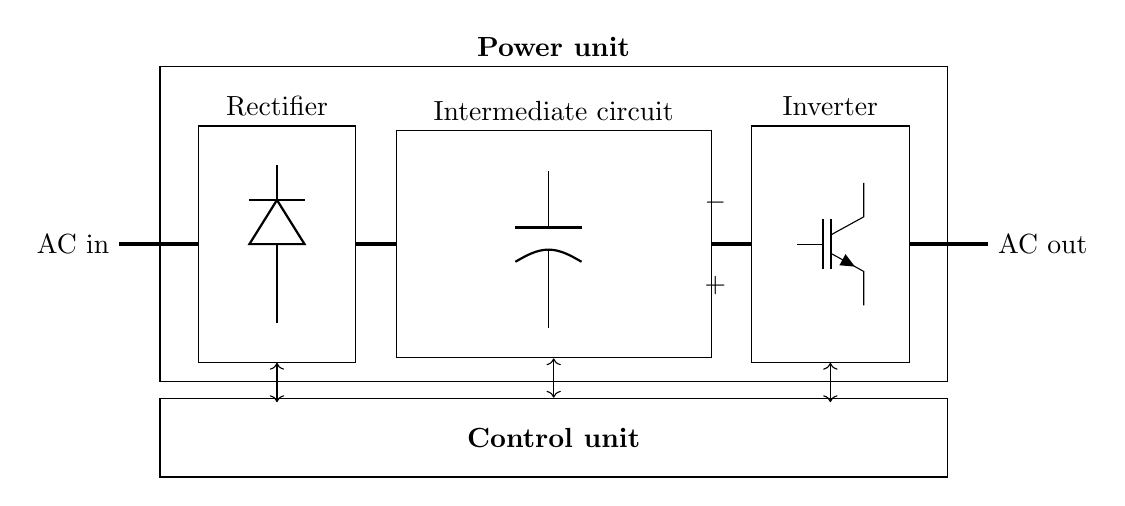
\begin{tikzpicture}[
	start chain=going right,
	box/.style={
		on chain,join,draw,
		minimum height=3cm,
		text centered,
		minimum width=2cm,
	},
	every join/.style={ultra thick},
	node distance=5mm
]

\node [on chain] {AC in}; % Chain starts here

\node [box,xshift=5mm,label=above:Rectifier] (rec) {
	\begin{circuitikz}
		\draw (0,0) to[Do] (0,2);
	\end{circuitikz}
};

\node [on chain,join,draw, 
	text width=1cm,
	minimum width=4cm,
	minimum height=1.6cm,
	label=above:Intermediate circuit,
] (ic) {
	\begin{circuitikz}[american voltages]
		\draw (0,0) to[pC,v>=$ $] (0,2);
	\end{circuitikz}
};

\node [box,label=above:Inverter] (inv) {
	\begin{circuitikz}
		\draw (0,0) node[nigbt] {};
	\end{circuitikz}
};

\node [on chain,join,xshift=5mm]{AC out};
% Chain ends here

% CU box
\node [
	rectangle,draw,
	below=5mm of ic,
	minimum width=10cm,
	minimum height=1cm,
] (cu) {\textbf{Control unit}};

% PU box
\node [
	rectangle,draw,
	above=2mm of cu,
	minimum width=10cm,
	minimum height=4cm,
	label=\textbf{Power unit},
] (pu) {};

% Connections between CU and PU
\draw[<->] (rec.south) -- ++(0,-5mm);
\draw[<->] (cu.north) to (ic.south);
\draw[<->] (inv.south) -- ++(0,-5mm);

\end{tikzpicture}



\chapter{Inserting Inline Codes} 
\label{AppendixD} 
\lhead{Appendix D. \emph{Inserting Inline Codes}} 

% Write your Appendix D content below here.
% ==============================================

\section{Formatting Source Codes}

% A complete reference manual can be found at \url{http://tug.ctan.org/tex-archive/macros/latex/contrib/listings/listings.pdf} \\
% \url{http://en.wikibooks.org/wiki/LaTeX/Source\_Code\_Listings} \\
% For writing software source codes in latex blocks of code. This is a basic example for listing program code: 
%% ALAILABLE LANGUAGE LISTINGS
%% http://tug.ctan.org/tex-archive/macros/latex/contrib/listings/listings.pdf#table.1
%% PREAMBLE SECTION MUST HAVE
%% \usepackage{listings}
% Set your language (you can change the language for each code-block optionally)
% The general form is \lstset{ language = [<dialect>] <language> }

Using small font

\lstset{basicstyle=\ttfamily\small} 
\begin{lstlisting}[breaklines, frame=single, numbers=left, caption={Create mylatex1.tex file using nano small font}, label=commandline-02]     

wruslan@wruslan-ub1404-fujitsuNB:~/latex01$ nano mylatex1.tex
wruslan@wruslan-ub1404-fujitsuNB:~/latex01$ ls -l
total 4
-rw-rw-r-- 1 wruslan wruslan 15 Oct 10 07:48 mylatex1.tex
wruslan@wruslan-ub1404-fujitsuNB:~/latex01$ cat mylatex1.tex 
Bismillah WRY.
wruslan@wruslan-ub1404-fujitsuNB:~/latex01$ 

\end{lstlisting}      

%\pagebreak

Using tiny font
    
\lstset{basicstyle=\ttfamily\tiny} 
\begin{lstlisting}[breaklines, frame=single, numbers=left, caption={Create mylatex1.tex file using nano tiny font}, label=commandline-02]     
wruslan@wruslan-ub1404-fujitsuNB:~/latex01$ nano mylatex1.tex
wruslan@wruslan-ub1404-fujitsuNB:~/latex01$ ls -l
total 4
-rw-rw-r-- 1 wruslan wruslan 15 Oct 10 07:48 mylatex1.tex
wruslan@wruslan-ub1404-fujitsuNB:~/latex01$ cat mylatex1.tex 
Bismillah WRY.
wruslan@wruslan-ub1404-fujitsuNB:~/latex01$ 
\end{lstlisting}      
        
    
\chapter{Inserting Inline Equations} 
\label{AppendixE} 
\lhead{Appendix E. \emph{Inserting Inline Equations}} 

% Write your Appendix content below here.
% =========================================

\section{Section Title}
To understand the \index{basic ideas} of software design Add and remove tabs Working with tabs in gedit allows you to keep an eye on several files in a single window. 

\subsection{subsection title}
The tab bla bla EQUATION

\begin{equation}
\binom{n+1}{k} = \binom{n}{k} + \binom{n}{k-1}
\end{equation}




\addtocontents{toc}{\vspace{2em}} 
% Add a gap in the Contents, for aesthetics

\backmatter

\end{document}  